
\chapter{Cyclopts Command Line Interface}\label{method:tools:cli}

Cyclopts provides a rich command line interface (CLI) for instance generation,
local execution, and remote execution. The CLI includes a number of useful
utilities, however this section will only present those required for running the
full Cyclopts workflow, both local and remote. The full set of CLI options is
presented in Listing \ref{lst:loptshlep}.

\lstinputlisting[
  style=BashOutputStyle,
  keywordstyle=\ttfamily,
  caption={All available Cyclopts CLI options (the result of \code{cyclopts -h}).}, 
  label=lst:loptshlep]{./backmatter/listings/help}

\section{Local Execution}

When working locally, the primary workflow is \code{cyclopts convert}, followed
by \code{cyclopts exec}, finishing with \code{cyclopts pp}. \code{cyclopts
  convert} converts a user-provided definition of a parameter space into an
instance database. \code{cyclopts exec} then executes some or all of those
instances, resulting in a solution database. Finally, \code{cyclopts pp}
post-processes the instance and solution data. The options for each are
described in Listings \ref{lst:loptsconvert}, \ref{lst:loptsexec}, and
\ref{lst:loptspp}, respectively.

\lstinputlisting[
  style=BashOutputStyle,
  keywordstyle=\ttfamily,
  caption={CLI options for \code{cyclopts convert}.}, 
  label=lst:loptsconvert]{./backmatter/listings/convert}

\lstinputlisting[
  style=BashOutputStyle,
  keywordstyle=\ttfamily,
  caption={CLI options for \code{cyclopts exec}.}, 
  label=lst:loptsexec]{./backmatter/listings/exec}

\lstinputlisting[
  style=BashOutputStyle,
  keywordstyle=\ttfamily,
  caption={CLI options for \code{cyclopts pp}.}, 
  label=lst:loptspp]{./backmatter/listings/pp}

A diagram explaining the role of the CLI workflow with respect to Cyclopts
object tree (as seen in Figure \ref{fig:lopts_desgin}) is shown below in Figure
\ref{fig:lopts_cli}.

\begin{figure}
  \begin{center}
    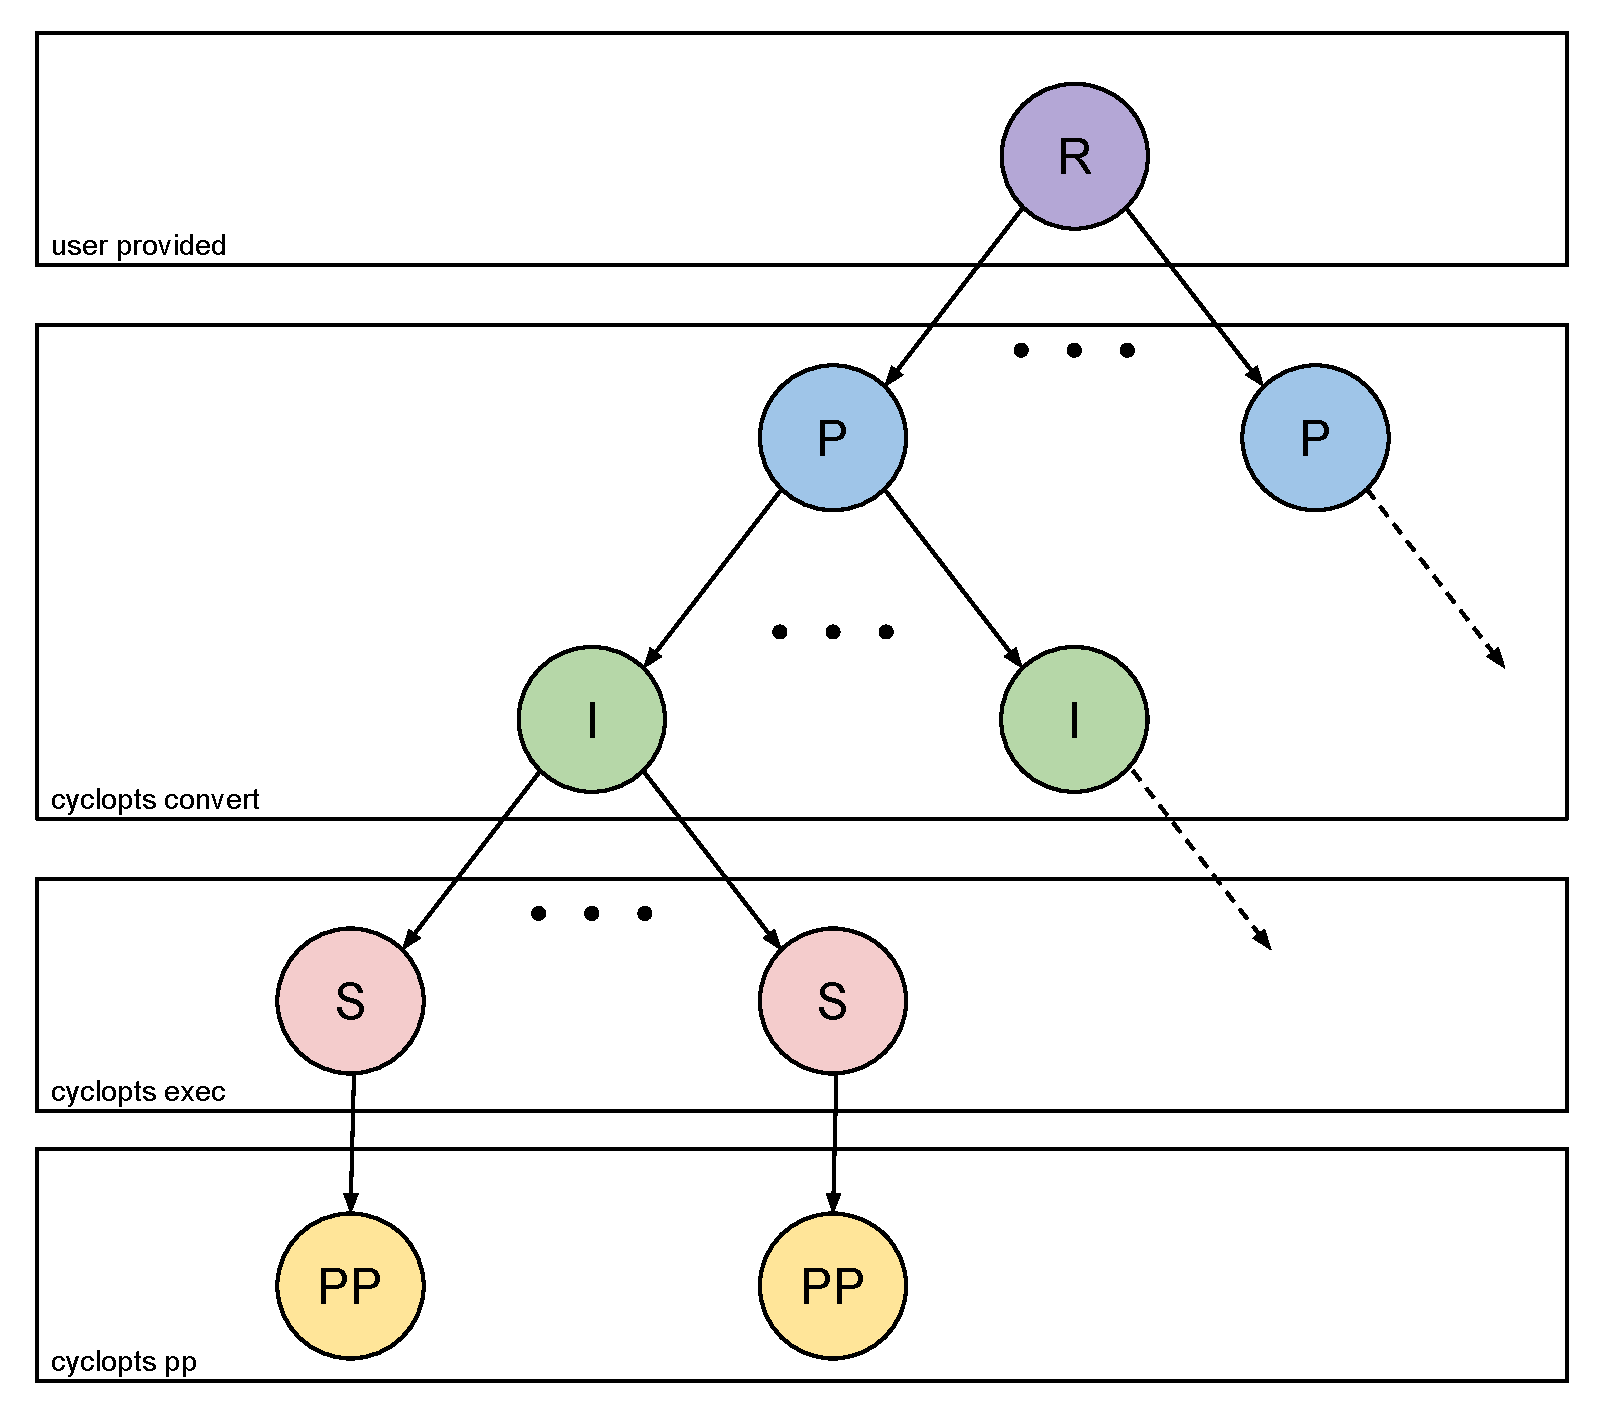
\includegraphics[width=\textwidth]{./backmatter/figs/cyclopts_tree_cli.pdf}
    \caption[]{
      \label{fig:lopts_cli}
      The Cyclopts object tree structure is shown with boxes around each group
      of objects that are created given a CLI call. Note that the root node is
      determined from user-provided input.}
  \end{center}
\end{figure}

\section{Remote Execution}

In order to execute Cyclopts on a Condor system, the submit node must contain
the Cyclopts environment. That operation is supported by the \code{cyclopts cde}
CLI, presented in Listing \ref{lst:loptscde}. A job, the input of which is an
instance database, can be submitted using \code{cyclopts condor-submit}. Upon
completion, results can be collected with \code{cyclopts condor-collect}. The
arguments for both are shown in Listings \ref{lst:loptscondor-submit} and
\ref{lst:loptscondor-collect}.

\lstinputlisting[
  style=BashOutputStyle,
  keywordstyle=\ttfamily,
  caption={CLI options for \code{cyclopts cde}.}, 
  label=lst:loptscde]{./backmatter/listings/cde}

\lstinputlisting[
  style=BashOutputStyle,
  keywordstyle=\ttfamily,
  caption={CLI options for \code{cyclopts condor-submit}.}, 
  label=lst:loptscondor-submit]{./backmatter/listings/condor-submit}

\lstinputlisting[
  style=BashOutputStyle,
  keywordstyle=\ttfamily,
  caption={CLI options for \code{cyclopts condor-collect}.}, 
  label=lst:loptscondor-collect]{./backmatter/listings/condor-collect}
